\documentclass[10pt]{article}  

%%%%%%%% PREÁMBULO %%%%%%%%%%%%
\title{Plantilla para prácticas de UPIITA}
\usepackage[spanish]{babel} %Indica que escribiermos en español
\usepackage[utf8]{inputenc} %Indica qué codificación se está usando ISO-8859-1(latin1)  o utf8  
\usepackage{amsmath} % Comandos extras para matemáticas (cajas para ecuaciones,
% etc)
\usepackage{amssymb} % Simbolos matematicos (por lo tanto)
\usepackage{graphicx} % Incluir imágenes en LaTeX
\usepackage{color} % Para colorear texto
\usepackage{subfigure} % subfiguras
\usepackage{float} %Podemos usar el especificador [H] en las figuras para que se
% queden donde queramos
\usepackage{capt-of} % Permite usar etiquetas fuera de elementos flotantes
% (etiquetas de figuras)
\usepackage{sidecap} % Para poner el texto de las imágenes al lado
	\sidecaptionvpos{figure}{c} % Para que el texto se alinie al centro vertical
\usepackage{caption} % Para poder quitar numeracion de figuras
\usepackage{commath} % funcionalidades extras para diferenciales, integrales,
% etc (\od, \dif, etc)
\usepackage{cancel} % para cancelar expresiones (\cancelto{0}{x})
 
\usepackage{anysize} 					% Para personalizar el ancho de  los márgenes
\marginsize{2cm}{2cm}{2cm}{2cm} % Izquierda, derecha, arriba, abajo

\usepackage{appendix}
\renewcommand{\appendixname}{Apéndices}
\renewcommand{\appendixtocname}{Apéndices}
\renewcommand{\appendixpagename}{Apéndices} 

% Para que las referencias sean hipervínculos a las figuras o ecuaciones y
% aparezcan en color
\usepackage[colorlinks=true,plainpages=true,citecolor=blue,linkcolor=blue]{hyperref}
%\usepackage{hyperref} 
% Para agregar encabezado y pie de página
\usepackage{fancyhdr} 
\pagestyle{fancy}
\fancyhf{}
\fancyhead[L]{\footnotesize UGR} %encabezado izquierda
\fancyhead[R]{\footnotesize EV}   % dereecha
\fancyfoot[R]{\footnotesize Práctica I}  % Pie derecha
\fancyfoot[C]{\thepage}  % centro
\fancyfoot[L]{\footnotesize Master en Ingeniería Informática}  %izquierda
\renewcommand{\footrulewidth}{0.4pt}


\usepackage{listings} % Para usar código fuente
\definecolor{dkgreen}{rgb}{0,0.6,0} % Definimos colores para usar en el código
\definecolor{gray}{rgb}{0.5,0.5,0.5} 
% configuración para el lenguaje que queramos utilizar
\lstset{language=Matlab,
   keywords={break,case,catch,continue,else,elseif,end,for,function,
      global,if,otherwise,persistent,return,switch,try,while},
   basicstyle=\ttfamily,
   keywordstyle=\color{blue},
   commentstyle=\color{red},
   stringstyle=\color{dkgreen},
   numbers=left,
   numberstyle=\tiny\color{gray},
   stepnumber=1,
   numbersep=10pt,
   backgroundcolor=\color{white},
   tabsize=4,
   showspaces=false,
   showstringspaces=false}

\newcommand{\sen}{\operatorname{\sen}}	% Definimos el comando \sen para el seno
%en español

%%%%%%%% TERMINA PREÁMBULO %%%%%%%%%%%%

\begin{document}

%%%%%%%%%%%%%%%%%%%%%%%%%%%%%%%%%% PORTADA %%%%%%%%%%%%%%%%%%%%%%%%%%%%%%%%%%%%%%%%%%%%
																					%%%
\begin{center}																		%%%
\newcommand{\HRule}{\rule{\linewidth}{0.5mm}}									%%%\left
 																					%%%
\begin{minipage}{0.48\textwidth} \begin{flushleft}
%
\includegraphics[scale = 0.63]{Imagenes/logo_upiita}
\end{flushleft}\end{minipage}
\begin{minipage}{0.48\textwidth} \begin{flushright}
%
\includegraphics[scale = 0.35]{Imagenes/IPN}
\end{flushright}\end{minipage}

													 								%%%
\vspace*{0.25cm}								%%%
																					%%%	
\textsc{\huge Universidad de Granada}\\[1.5cm]	

\textsc{\LARGE Master en Ingeniería Informática}\\[1.5cm]													%%%

\textsc{\LARGE Entornos Virtuales}\\[1.5cm]													%%%

\begin{minipage}{0.9\textwidth} 
\begin{center}																					%%%
\textsc{\LARGE Practica I}
\end{center}
\end{minipage}\\[0.5cm]
%%%
    																				%%%
 			\vspace*{1cm}																		%%%
																					%%%
\HRule \\[0.4cm]																	%%%
{ \huge \bfseries Modelado con Blender}\\[0.4cm]	%%%
 																					%%%
\HRule \\[1.5cm]																	%%%
 																				%%%
																					%%%
\begin{minipage}{0.46\textwidth}													%%%
\begin{flushleft} \large															%%%
\emph{Autor:}\\	
 Manuel Jesús García Manday
%%%
			%\vspace*{2cm}	
            													%%%
										 						%%%
\end{flushleft}																		%%%
\end{minipage}		
																%%%
\begin{minipage}{0.52\textwidth}		
\vspace{-0.6cm}											%%%
\begin{flushright} \large															%%%													%%%
\end{flushright}																	%%%
\end{minipage}	
\vspace*{1cm}
%\begin{flushleft}
 	
%\end{flushleft}
%%%
 		\flushleft{\textbf{\Large Master en Ingeniería Informática}	}\\																		%%%
\vspace{2cm} 																				
\begin{center}																					
{\large \today}																	%%%
 			\end{center}												  						
\end{center}							 											
																					
\newpage																		
%%%%%%%%%%%%%%%%%%%% TERMINA PORTADA %%%%%%%%%%%%%%%%%%%%%%%%%%%%%%%%

\tableofcontents 

\newpage

\section{Objetivo.}

El objetivo de esta primera práctica es el de realizar el modelado de una figura mediante Blender, empleando para ellos las técnicas y procedimientos necesarios vistos en el guión de la misma.



\section{Figura a modelar.} 

Se ha seleccionado la figura de la imagen que se  muestra a continuación para realizar el modelado.

\begin{figure}[H]
	\begin{center}
	 		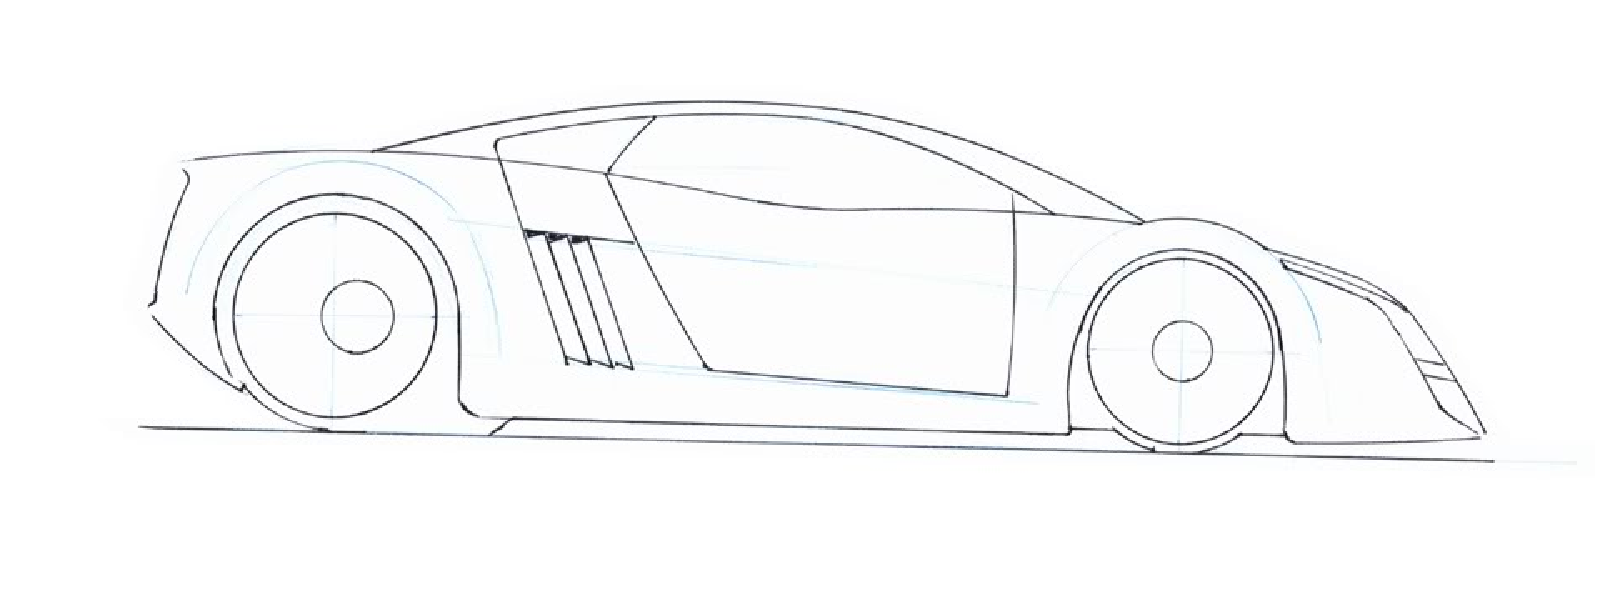
\includegraphics[width = 0.5\textwidth]{Imagenes/dibujoCoche.eps}
 		\captionof{figure}{\label{fig:IPN}Imagen a modelar} 
	\end{center} 
\end{figure}


\section{Desarrollo de la práctica.}


A partir de la imagen anterior se comenzará a realizar el modelado de la misma. Partimos del cubo que por defecto crea Blender al iniciarse y colocando la imagen de fondo empezamos a darle forma al cubo expandiendolo horizontalmente y verticalmente hasta que cubra todo el espacio que ocupa la figura, es decir, el objeto será redimensionado en los ejes X e Y.

Una vez que el modelo del cubo ha cubierto toda la figura, pasamos a crearnos cadenas de aristas que vayan pasando por las zonas delimitadas por la imagen. Se van añadiendo aristas en ambos ejes (X e Y) y se van editando los vertices que se crean por las intersecciones de las aristas para que coincidan con la figura de la imagen.

Con la malla de polígonos terminada pasamos a aplicarle uno de los modificadores utilizados para realizar el modelado, el modificador  \textbf{mirror}. Lo primero que hacemos es trazar una arista horizontal y eliminar la mitad del modelo como se muestra en la siguiente imagen.\\

\begin{figure}[H]
	\begin{center}
 		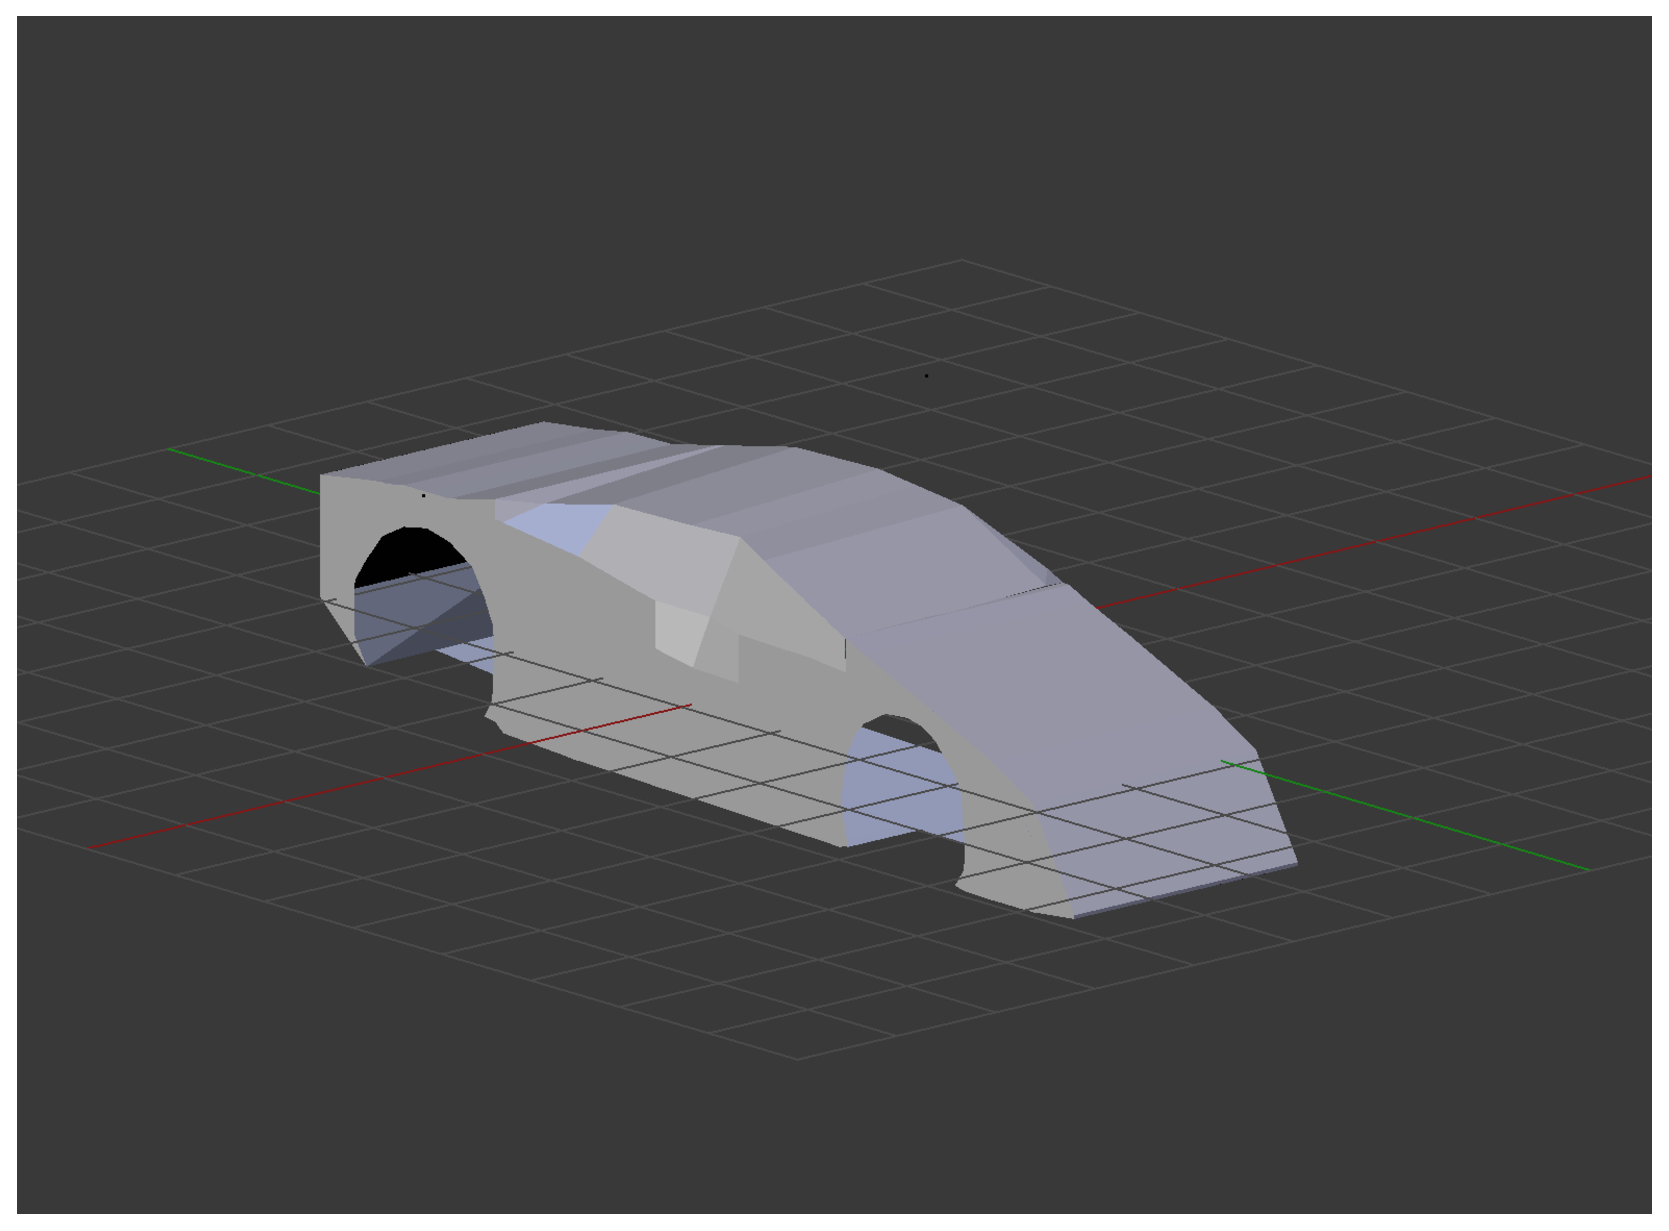
\includegraphics[width = 0.5\textwidth]{Imagenes/mirror.eps}
 		\captionof{figure}{\label{fig:IPN}Modificador mirror (I)} 
	\end{center} 
\end{figure}


Al aplicar dicho modificador la parte que se ha borrado del modelo se autocompleta quedando como una imagen espejo de la otra, de manera que cualquier característica o técnica que se aplique a la parte existente, es decir, la que no se ha eliminado, se verá reflejada en la parte creada a partir del modificador. \\

\begin{figure}[H]
	\begin{center}
 		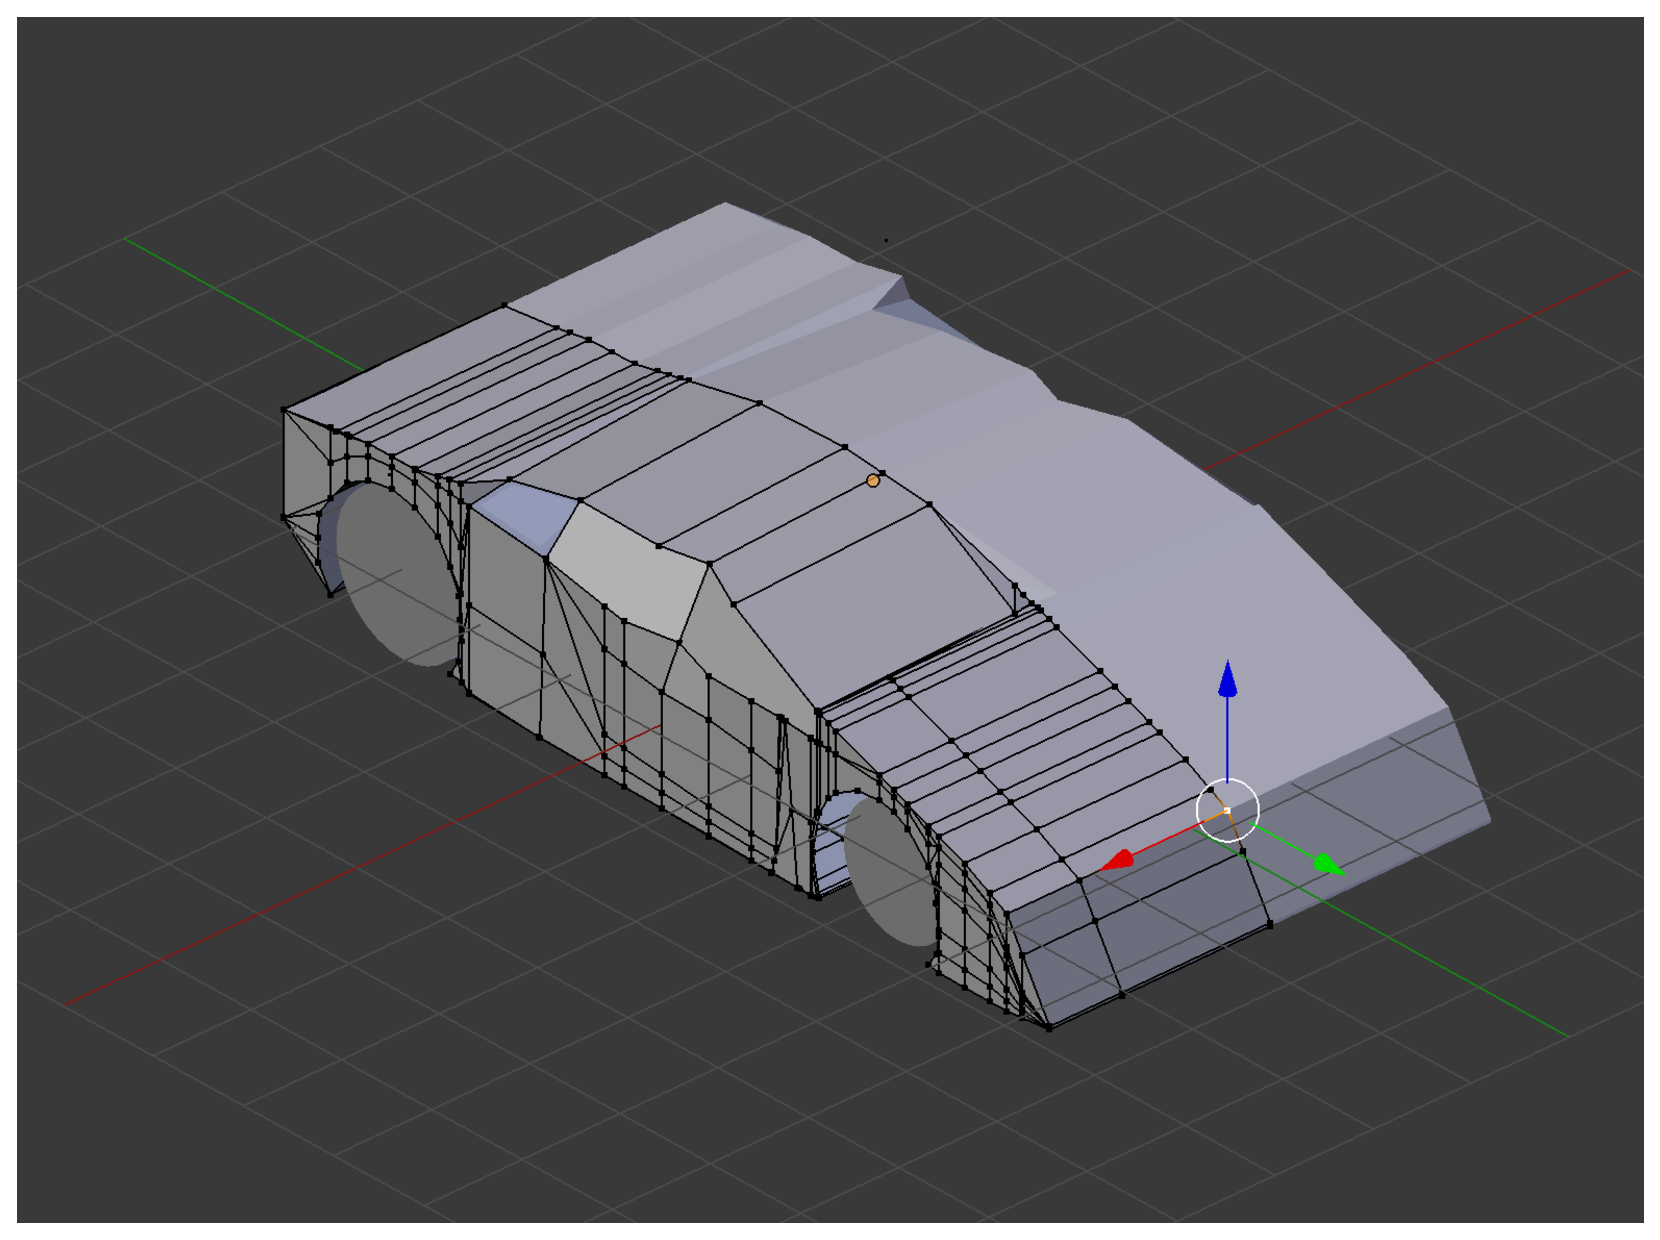
\includegraphics[width = 0.5\textwidth]{Imagenes/mirror2.eps}
 		\captionof{figure}{\label{fig:IPN}Modificador mirror (II)} 
	\end{center} 
\end{figure}

\begin{figure}[H]
	\begin{center}
 		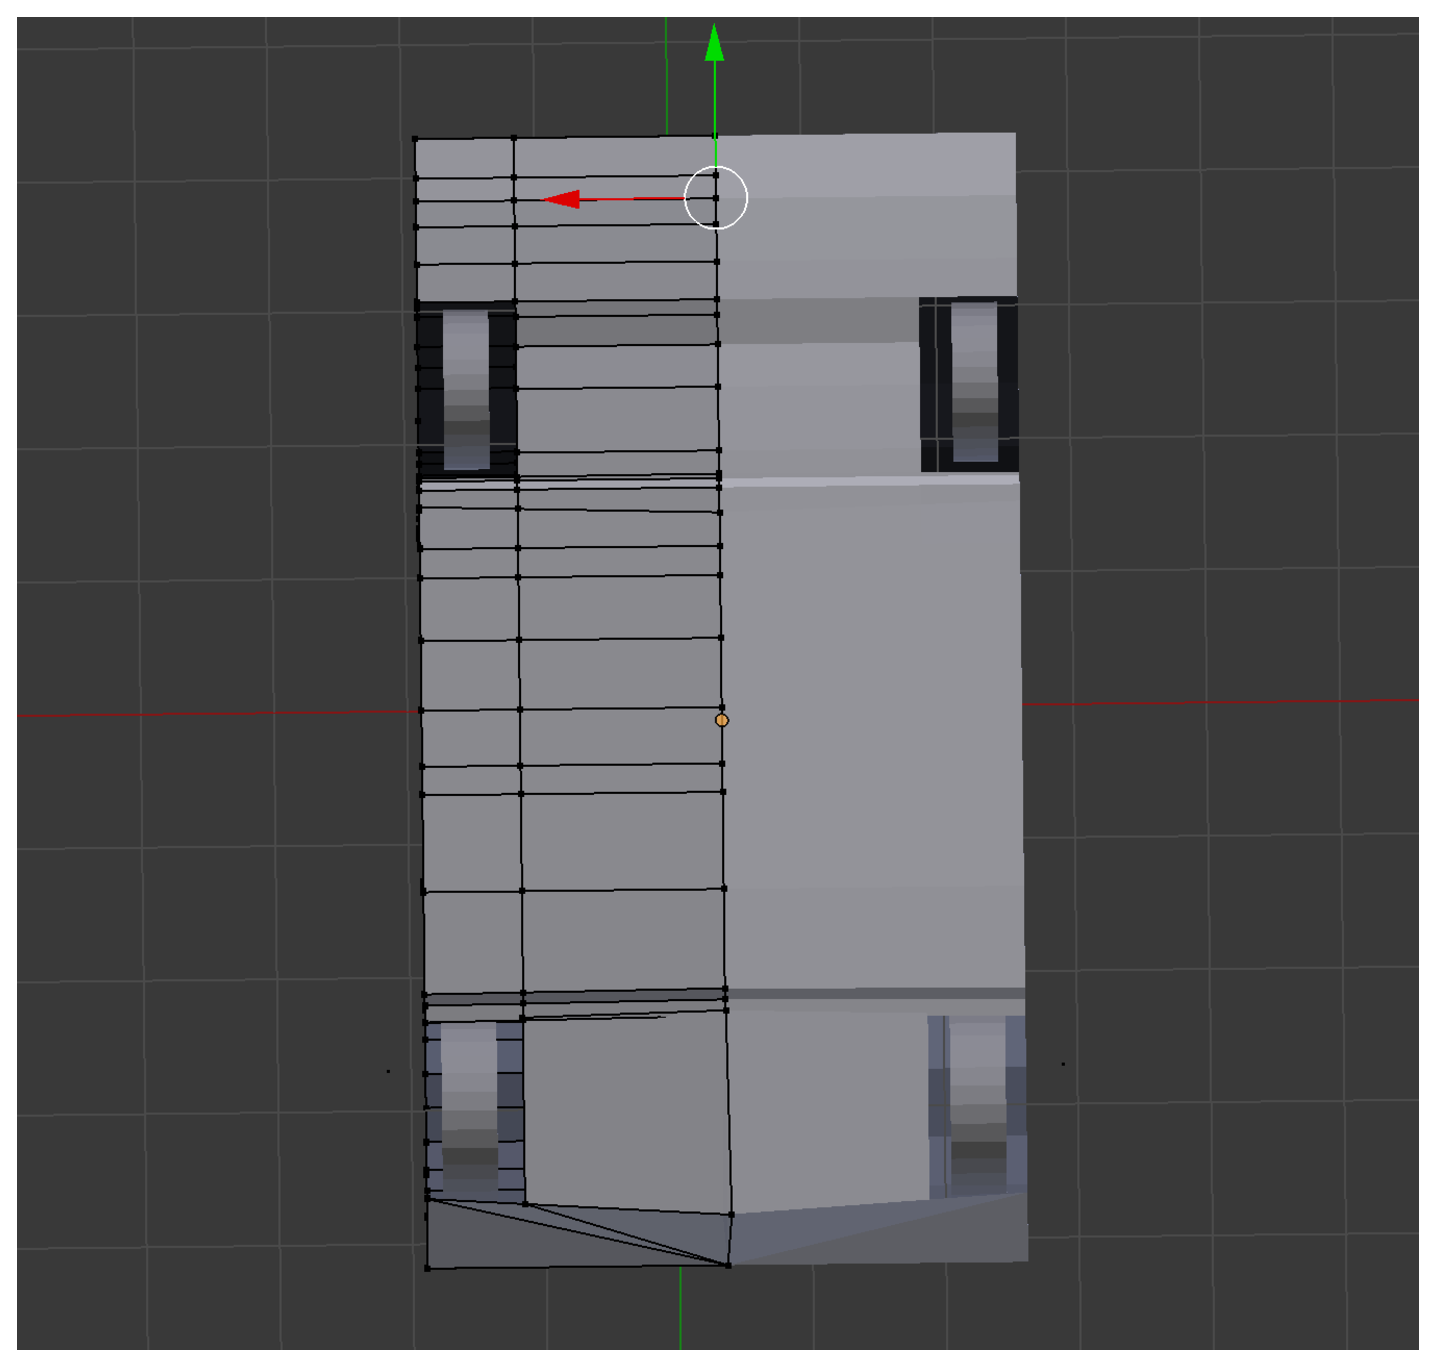
\includegraphics[width = 0.5\textwidth]{Imagenes/mirror3.eps}
 		\captionof{figure}{\label{fig:IPN}Modificador mirror (y III)} 
	\end{center} 
\end{figure}

Además del mencionado, se ha echo también uso del modificador  \textbf{subdivision surface} para crear curvaturas y parecer de esta redondeado, permitiendo así mostrar un mayor realismo.\\

Se han utilizado dos cilindros para crear las cuatro ruedas. A ambos se le han aplicado las transformaciones geométricas correspondientes de escalado, rotación y translación para que se ajusten al modelo de la figura. Una vez terminadas las transformaciones, diferentes en cuanto a parámetros, se han duplicado para tener definitivamente las dos ruedas delanteras y las dos ruedas traseras. \\

En la creación de las ventanas laterales y la luna delantera se ha empleado el mecanismo de  \textbf{extrusión} para la creación de dichos objetos a partir de los ya existentes, como es el techo del coche y las puertas laterales. Técnicas como la subdivisión de aristas para conseguir otro vértice intermedio ha sido también utilizada en el desarrollo del modelado.\\

Junto con todas esas técnicas mencionadas anteriormente, hay que añadir las de editado de vértices, aristas y caras, la eliminación también de estas, asi como la creación de caras a partir de un conjunto de vértices o aristas.\\


\subsection{Técnicas y renderizado.}

Todas estas técnicas mencionadas en el apartado anterior pueden verse reflejadas en las siguientes imágenes:

\begin{figure}[H]
	\begin{center}
 		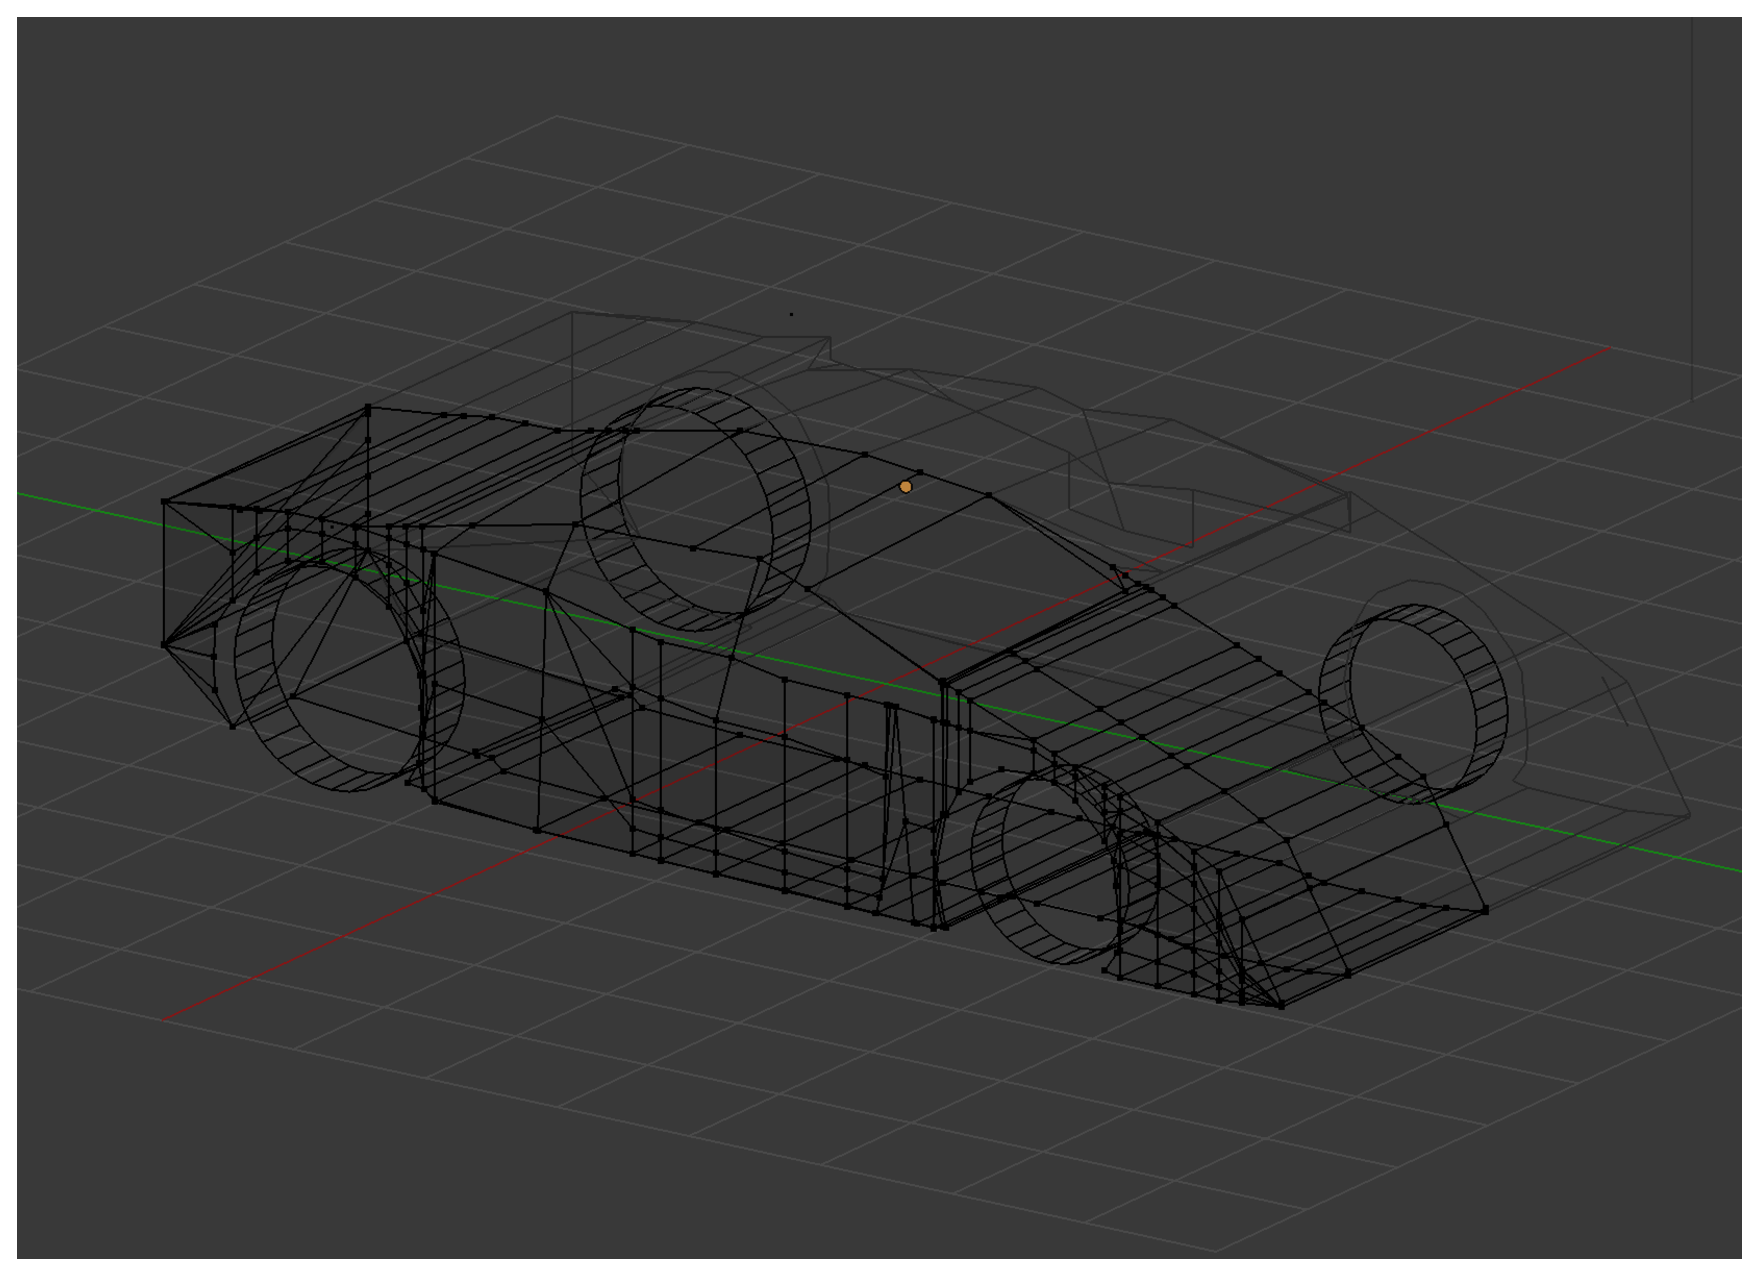
\includegraphics[width = 0.5\textwidth]{Imagenes/modelVertex.eps}
 		\captionof{figure}{\label{fig:IPN}Modelado en vértices} 
	\end{center} 
\end{figure}

\begin{figure}[H]
	\begin{center}
 		\includegraphics[width = 0.5\textwidth]{Imagenes/modelEdges.eps}
 		\captionof{figure}{\label{fig:IPN}Modelado en aristas} 
	\end{center} 
\end{figure}

\begin{figure}[H]
	\begin{center}
 		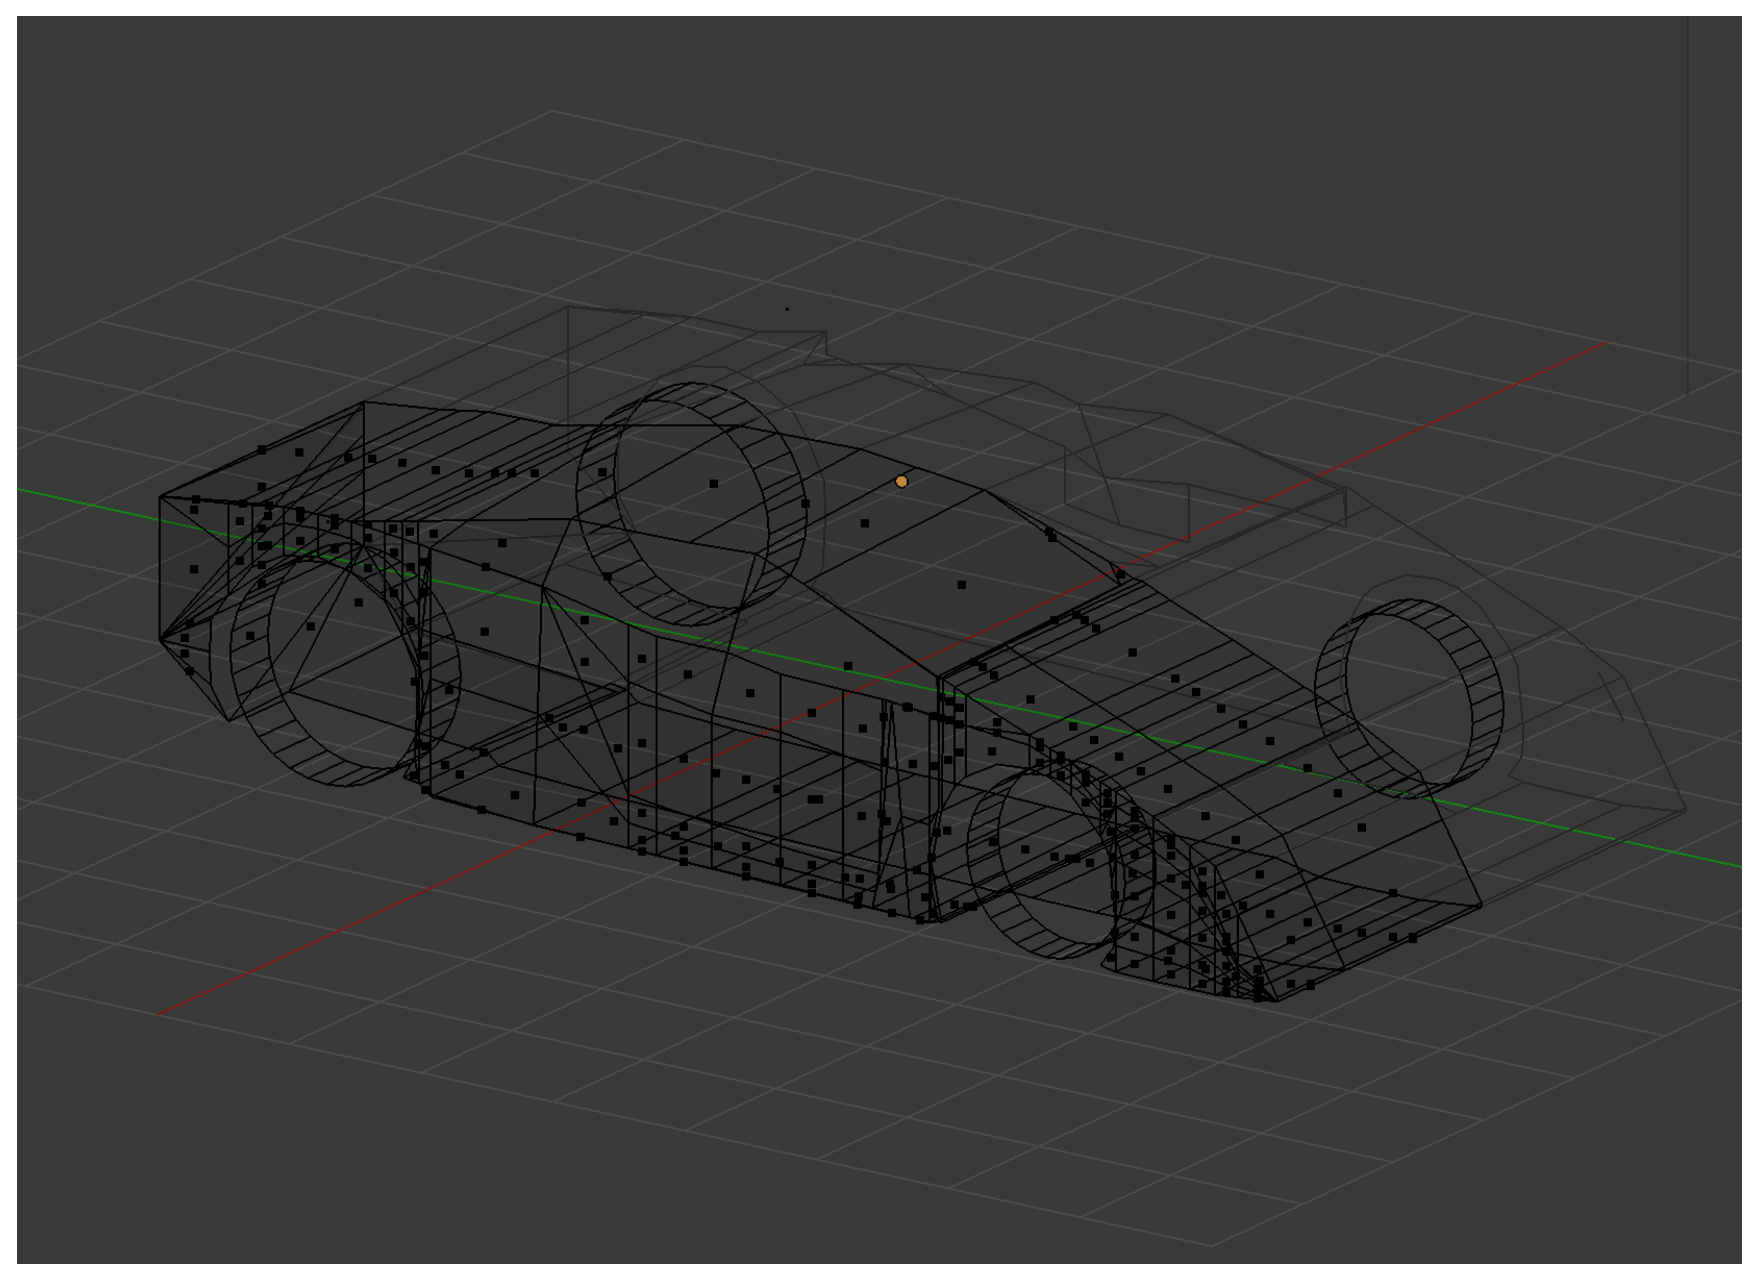
\includegraphics[width = 0.5\textwidth]{Imagenes/modelFaces.eps}
 		\captionof{figure}{\label{fig:IPN}Modelado en caras} 
	\end{center} 
\end{figure}

\begin{figure}[H]
	\begin{center}
 		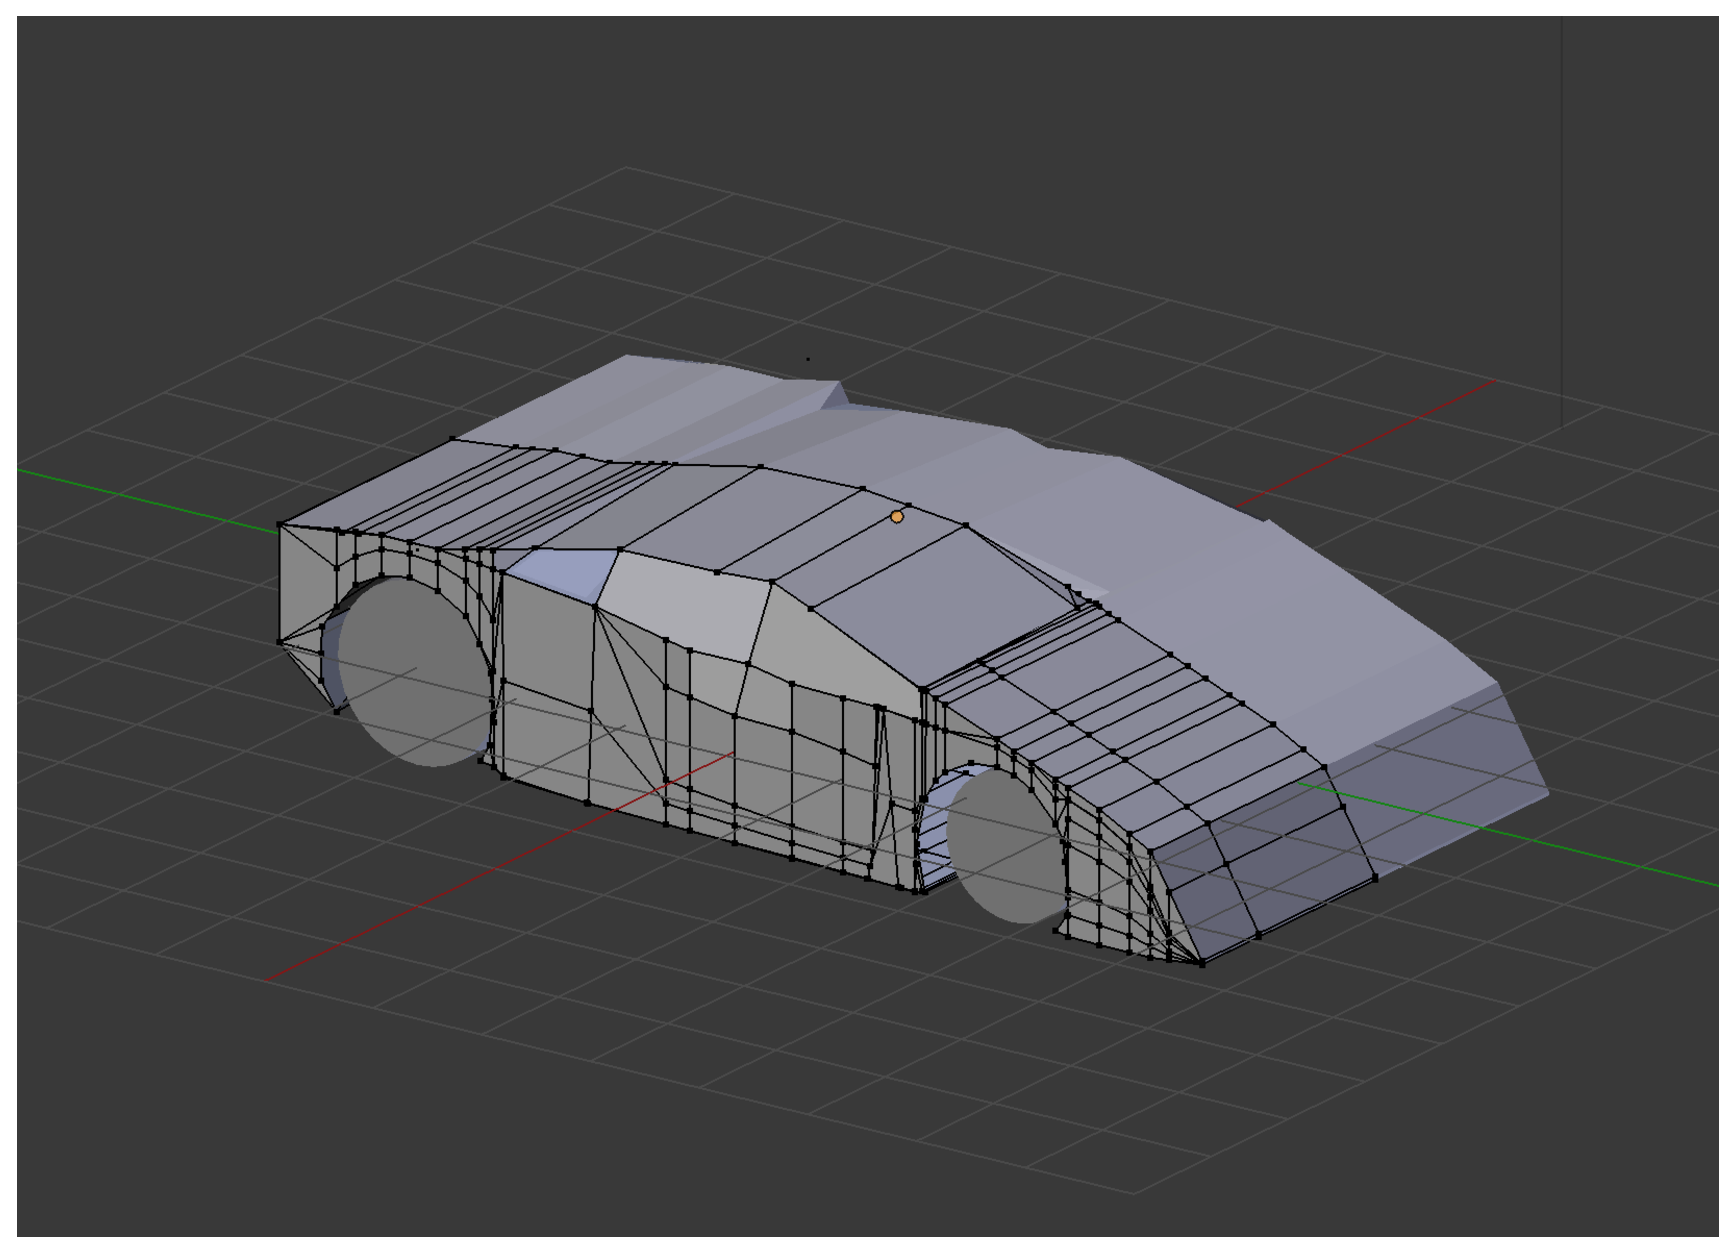
\includegraphics[width = 0.5\textwidth]{Imagenes/modelSolidVertex.eps}
 		\captionof{figure}{\label{fig:IPN}Modelado sólido en vértices} 
	\end{center} 
\end{figure}

\begin{figure}[H]
	\begin{center}
 		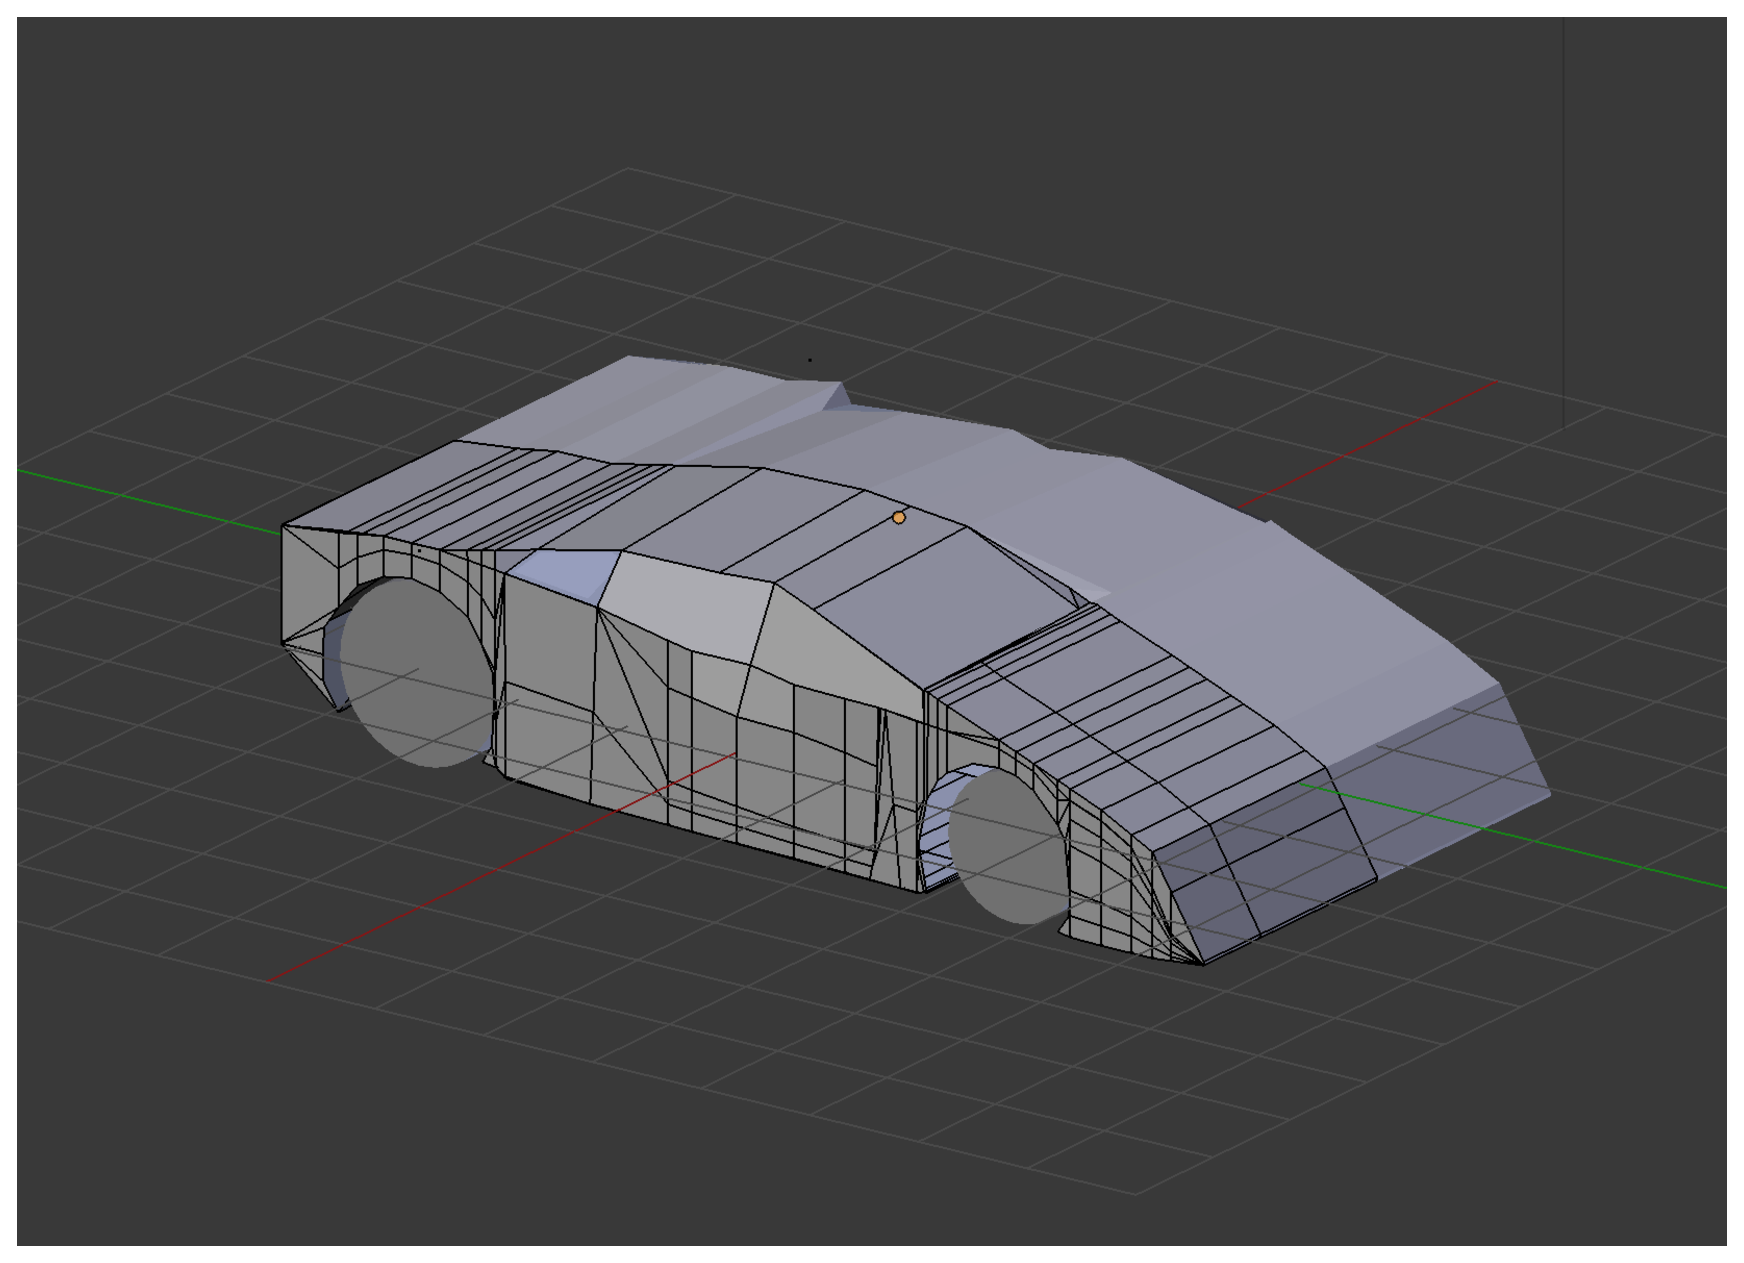
\includegraphics[width = 0.5\textwidth]{Imagenes/modelSolidEdges.eps}
 		\captionof{figure}{\label{fig:IPN}Modelado sólido en aristas} 
	\end{center} 
\end{figure}

\begin{figure}[H]
	\begin{center}
 		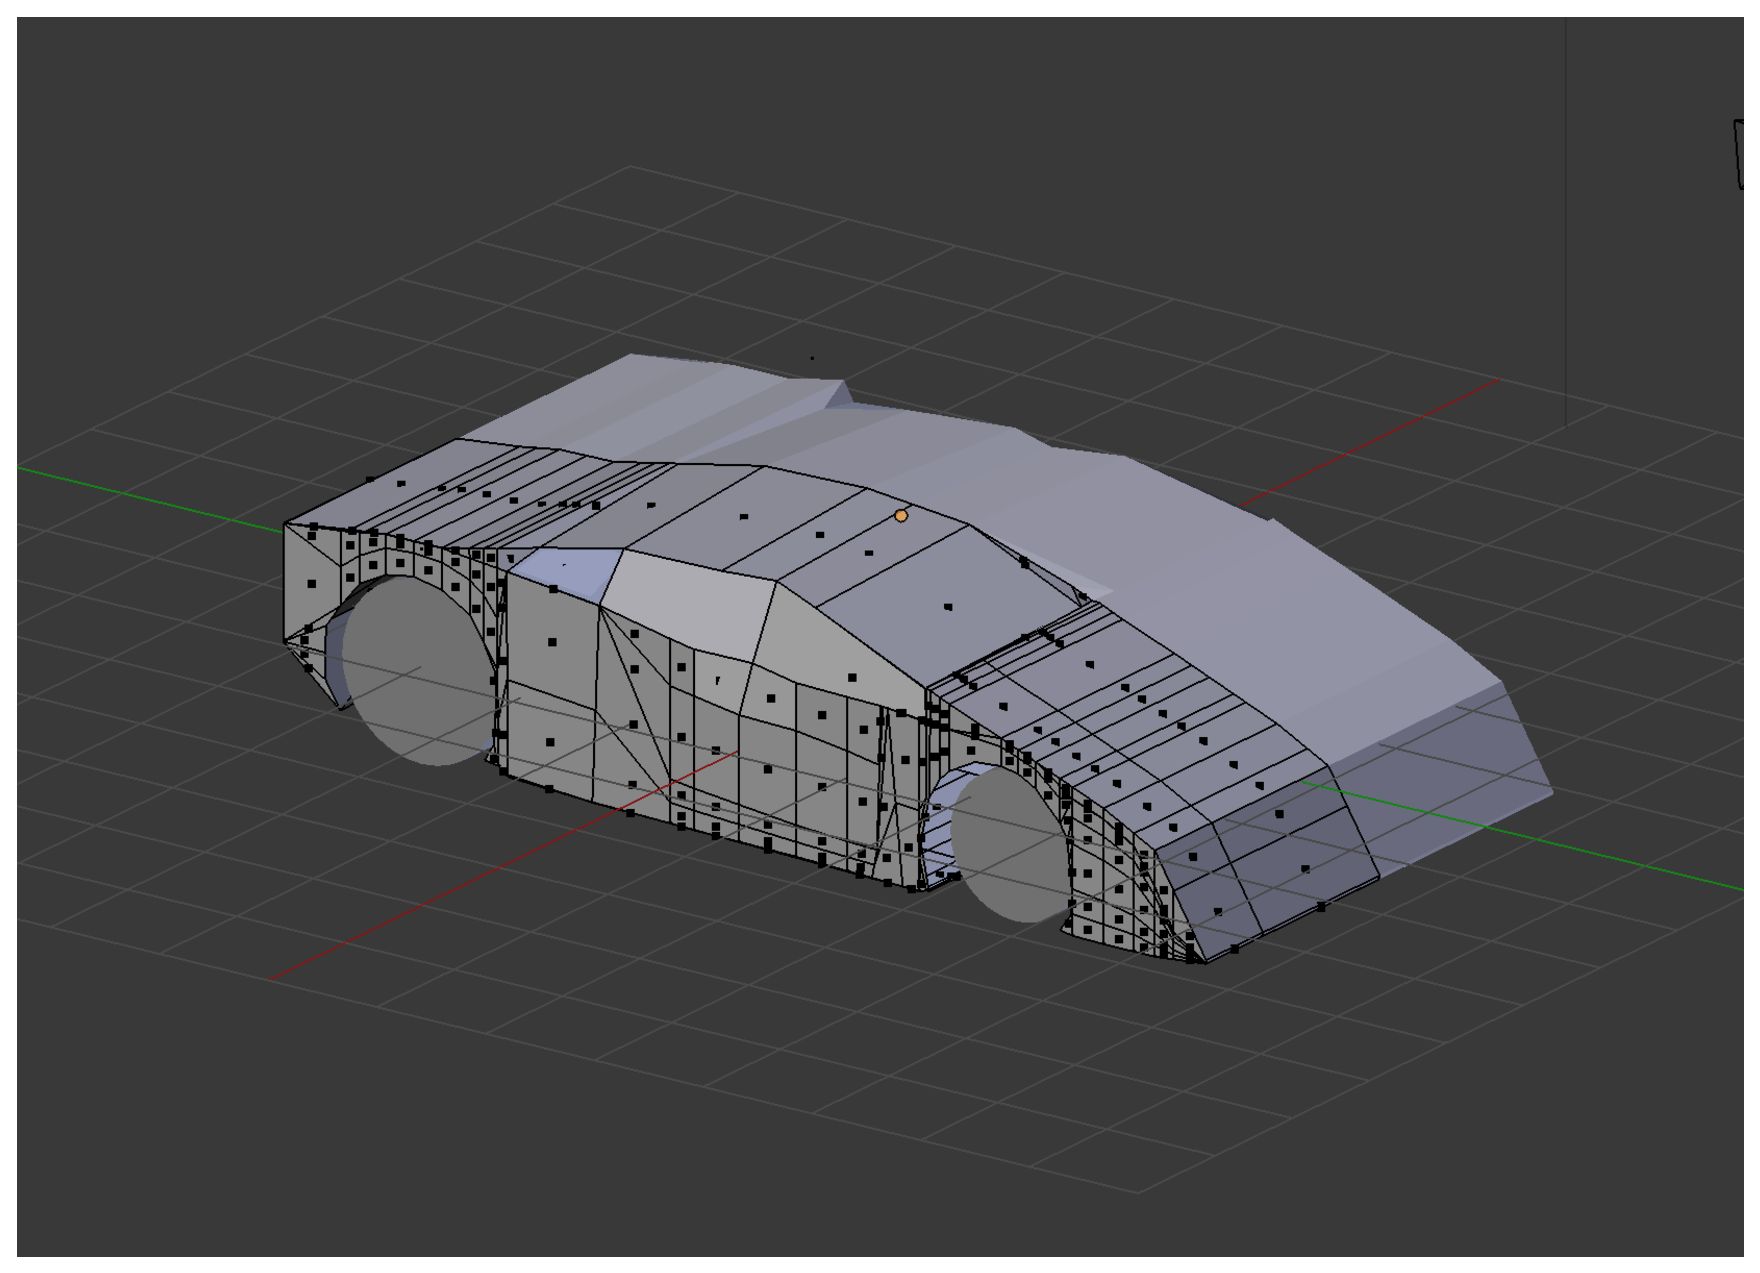
\includegraphics[width = 0.5\textwidth]{Imagenes/modelSolidFaces.eps}
 		\captionof{figure}{\label{fig:IPN}Modelado sólido en caras} 
	\end{center} 
\end{figure}

Antes de pasar al renderizado hay una característica a comentar para que no pase por alto, y es referente al modificador \textbf{subdivision surface}, el cual no es muy recomensable asignarle al parámetro view un índice alto, ya que esto provocaría un aumento en el número de divisiones y por consiguiente un mayor número de caras en la malla de polígonos, creciendo por tanto el tiempo en el renderizado. Para esta práctica se ha establecido el parámetro view a 2, que es un índice recomensable. \\

Con el modelado realizado y los parámetros configurados correctamente el resultado de realizar el renderizado es el que muestra la imagen:\\

\begin{figure}[H]
	\begin{center}
 		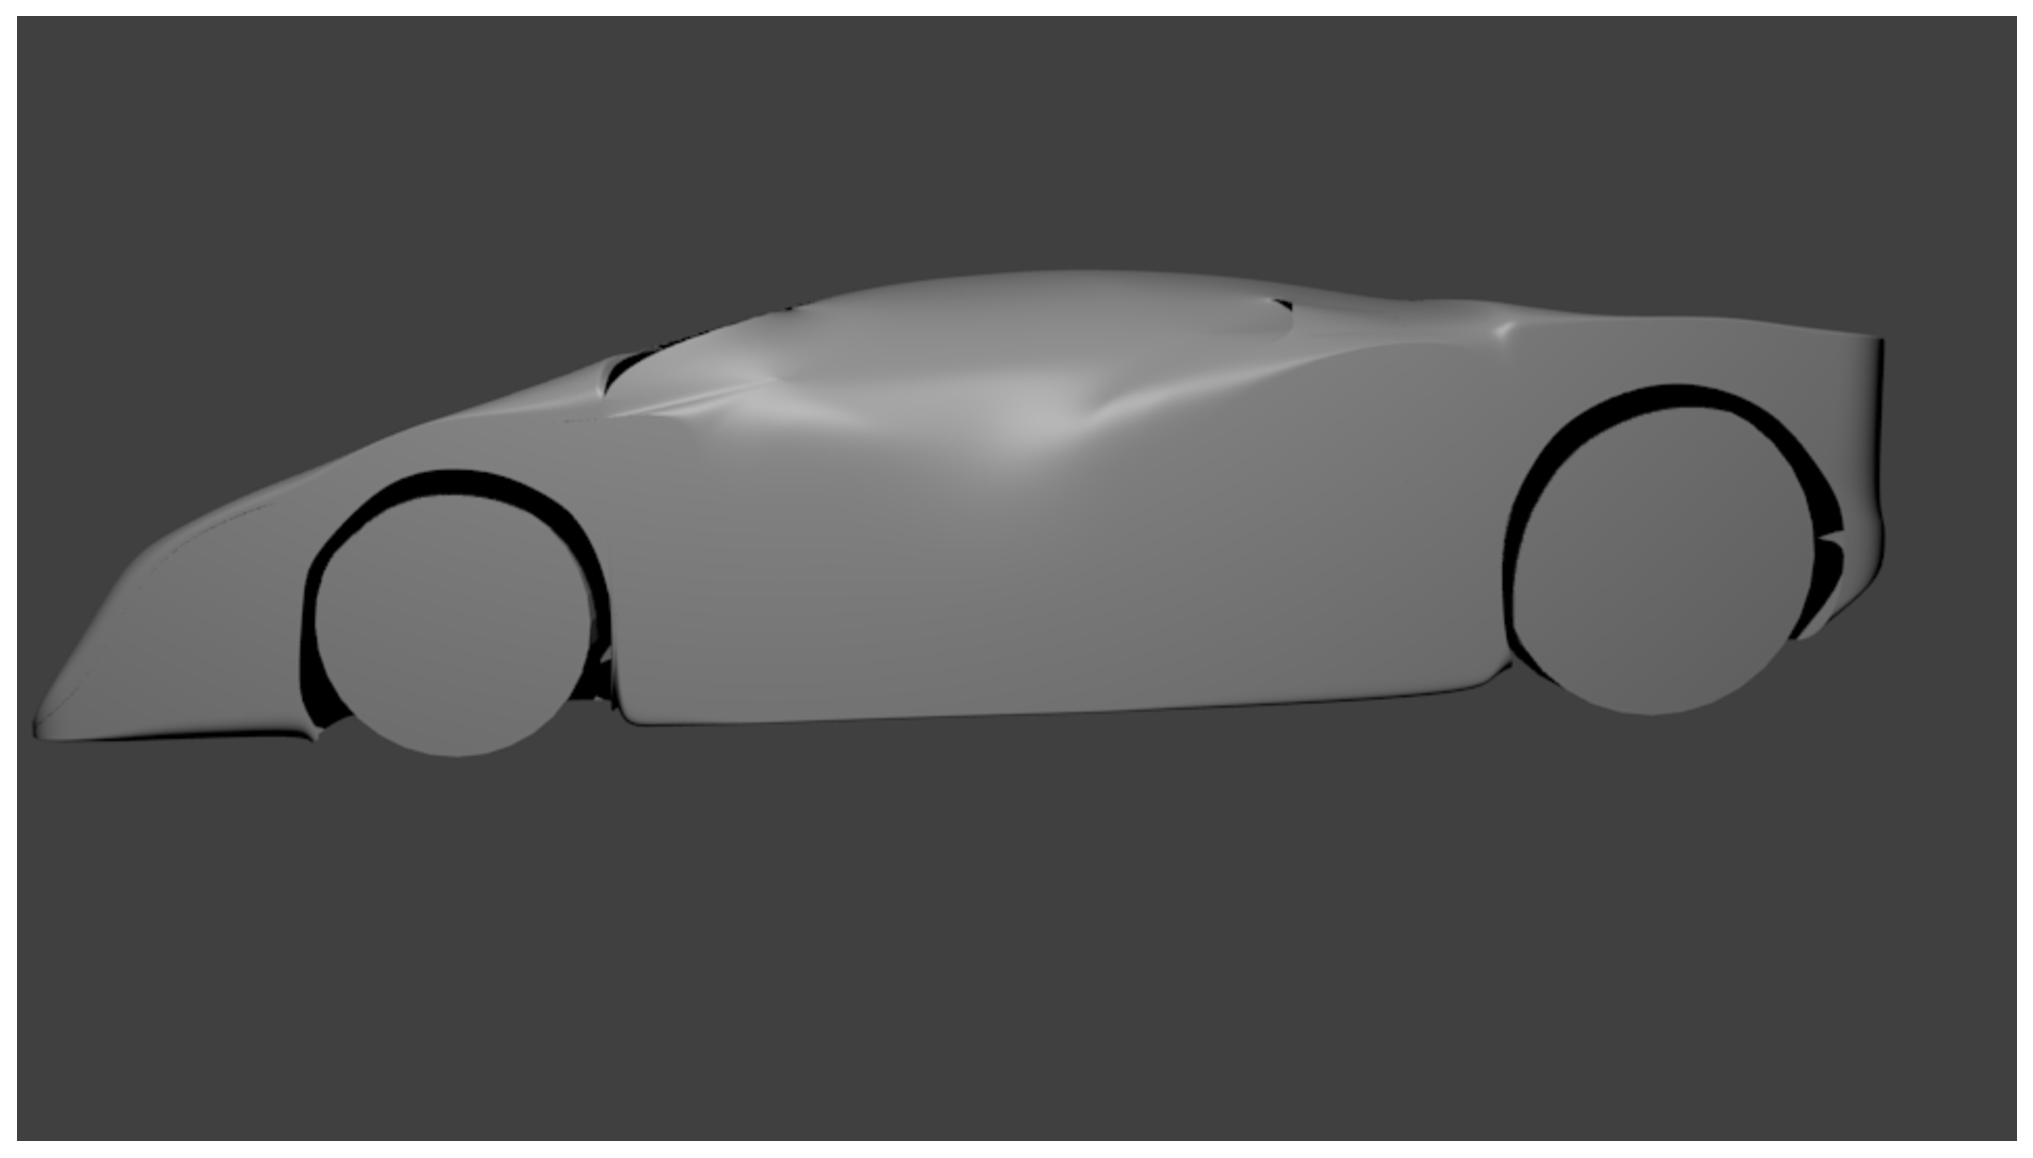
\includegraphics[width = 0.5\textwidth]{Imagenes/render.eps}
 		\captionof{figure}{\label{fig:IPN}Modelado sólido en caras} 
	\end{center} 
\end{figure}

En el documento zip referente a la entrega de la práctica se encuentra la imagen del renderizado, así como el fichero de blender correspondiente a la misma y la memoria de la misma.

\end{document}